\section{Trapdoor Claw Free Functions - TCFs} \label{tfcs}

\subsection{One-way function}
Informally, one-way functions are functions that are ``easy'' to compute but ``hard'' to invert in a ``computational sense.'' With these special properties, one-way functions are among the most fundamental tools for building classical and post-quantum cryptographic protocols, ranging from authentication, and signature to public key encryption schemes. 

\begin{defn}[One-way function]
    A function $f:\{0,1\}^* \to \{0,1\}^*$ is called one-way if two conditions hold:
    \begin{itemize}
        \item \textbf{Easy to compute}: There exists a polynomial-time algorithm that, on input $x$, outputs $f(x)$.
        \item \textbf{Hard to invert}: For every probabilistic polynomial-time algorithm $\mathcal{A}$, given $f(x)$, the probability that $\mathcal{A}$ finds a preimage of $f(x)$ is negligible, i.e.,
        \begin{align}
            \Pr[\mathcal{A}(f(x)) \in f^{-1}(f(x))] = \mathsf{negl}(\cdot).
        \end{align}
    \end{itemize}
\end{defn}

\noindent Given a one-way function $f(x)$, one question is raised: \textit{does the output of a one-way function, $y=f(x)$, truly conceal all information of the preimage $x\in f^{-1}(f(x))$?} The answer is NO! 
Consider $x=x_1\dots x_n$ and assuming that $g(x)$ is another one-way function, it follows that $f(x) = x_1||g(x)$ remains a one-way function since an adversary $\mathcal{A}$ must still invert $g(x)$ to determine the whole $x$. The first bit $x_1$ does not reveal information about other bits of $x$, as $x$ is sampled uniformly at random. This example illustrates the fact that the output of a one-way function could reveal some information about a certain bit of $x$.

Hence, we need a Boolean predicate (a Boolean function) $\mathcal{B}:\{0,1\}^*\to\{0,1\}$ that is completely hidden given the output of a one-way function. This leads us to the definition of the hardcore bit property.

\noindent More formally, the hardcore bit property (or hard-core predicate) ensures that even with the information of $y=f(x)$, guessing $\mathcal{B}(x)\in\{0,1\}$ is as challenging as finding $x$. 

\begin{defn}[Hardcore bit property]
    $\mathcal{B}:\{0,1\}^*\to\{0,1\}$ is a hardcore bit predicate of a one way function $f:\{0,1\}^*\to\{0,1\}^*$ if
    \begin{itemize}
        \item $\mathcal{B}$ is efficiently computable,
        \item It is “hard" to compute a bit $\mathcal{B}(x)$ of $x$ given $f(x)$. Formally, for all adversaries $\mathcal{A}$
        $$\Pr_{x\gets\{0,1\}^*}[\mathcal{A}(f(x))=\mathcal{B}(x)]\leq \displaystyle\frac{1}{2}+\mathsf{negl}(\cdot).$$
    \end{itemize}
\end{defn}


\subsection{Trapdoor Claw Free Functions}

In this section, we recall the definition of the trapdoor claw-free functions~\cite{GRM85},~\cite{Brakerski18_Interactiveproofofquantumness}.

\begin{figure}[!htb]
	\centering
	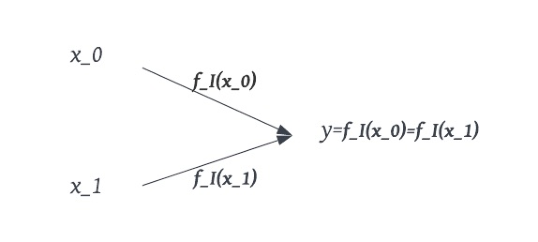
\includegraphics[]{figures/TCF.pdf}
	\caption{``A claw'' of a TCF function $f_{\mathcal{I}}(x)$ is a pair of $(x_0,x_1)$ such that $y=f_{\mathcal{I}}(x_0)=f_{\mathcal{I}}(x_1)$}\label{fig:TCF}
\end{figure}


Trapdoor claw-free functions (TCF), Fig.~\ref{fig:TCF}, is a 2-to-1 one-way function $f_\mathcal{I}(x)$ such that it is hard for a (quantum) polynomial-time adversary to simultaneously find the preimage pair $(x_0,x_1)$ \textit{``a claw''}, given any image $y = f_{\mathcal{I}}(x_0)=f_{\mathcal{I}}(x_1)$ where $\mathcal{I}$ is some problem instance. Sometimes, TCFs can also be defined as a pair of functions $f_{\mathcal{I},0}(x)$, $f_{\mathcal{I},1}(x)$ that are both injective and have the same image space and it is cryptographically hard to find two inputs mapping to the same output. One special property of TCFs is that given a problem instance $\mathcal{I}$ sampled together with a suitable trapdoor $t_{k}$, it is possible for one to find all the pre-images of $y$. More formally, we can define the trapdoor claw-free function as follows:
\begin{defn}[Trapdoor Claw-Free Function (TCF)]
    Let $\mathcal{X}$, $\mathcal{Y}$ be finite sets, we require the family of functions $\mathcal{F}$ satisfies the following properties:
\begin{itemize}
    \item For each public key $k$, there are two functions $\{f_{\mathcal{I},b}:\mathcal{X}\to\mathcal{Y}\}_{b\in\{0,1\}}$ that are both injective and have the same range, and are invertible given a suitable trapdoor $t_k$ (i.e.  $t_k$ can be used to efficiently compute $x$ given $b$ and $y=f_{\mathcal{I},b}(x)$). 
    \item The pair of functions should be \textit{claw-free}: it is hard to find the pair $(x_0,x_1)\in\mathcal{X}^2$ such that $y=f_{k,0}(x_0)=f_{k,1}(x_1)$.
\end{itemize}
\end{defn}

\noindent Note that a quantum device can not invert the function a find the claw $(x_0,x_1)$, it can hold these two preimages together with $y$ in a superposition
\begin{align}
    \frac{1}{\sqrt{2}}(\ket{x_0}+\ket{x_1})\ket{y}.
    \label{eq:tcfstate}
\end{align}
This is obtained by first preparing a uniform superposition over all $x\in\mathcal{X}$ via Hadamard transform
\begin{align}
    \frac{1}{\sqrt{\mathcal{X}}}\sum_{x\in\mathcal{X}}\ket{x},
\end{align}
then evaluating $f_{\mathcal{I},b}(x)$ into an output register to yield 
\begin{align}
    \frac{1}{\sqrt{\mathcal{X}}}\sum_{x\in\mathcal{X}}\ket{x}\ket{f_{\mathcal{I},b}(x)}.
\end{align}
If one measures the output register and obtains the result $y$, the state would collapse to the~\eqref{eq:tcfstate} state such that $y=f_{k,0}(x_0)=f_{k,1}(x_1)$.
Measuring the~\eqref{eq:tcfstate} state in the standard basis ($Z$ basis), one would obtain a random preimage as the measurement result, i.e. $m=x_0$ or $m = x_1$, but not both, since measuring a quantum state means collapsing that state to one possible outcome. Besides, measuring ~\eqref{eq:tcfstate} state in the $X$ basis yields a measurement result $m$ and a bit $c$ that satisfy $m \cdot (x_0\oplus x_1) = c$. This special property of TCFs could be used to construct a Proof of Quantumness protocol, the details of which will be discussed in section~\ref{proof_of_quantumness}.



However, a fully constructive Trapdoor Claw-Free (TCF) function that satisfies our cryptographic requirements has not been explored yet. The paper \cite{Brakerski18_Interactiveproofofquantumness} considers a ``relaxed'' version of the TCFs, referred to as \textbf{Noisy trapdoor claw-free functions (NTCFs)}. In NTCFs, the range of functions $f_{k,0}$ and $f_{k,1}$ is represented by a distribution $\mathcal{D}$ over $\mathcal{Y}$, denoted as $\mathcal{D}_{\mathcal{Y}}$. In other words, each function returns a density rather than a point. Instead of considering the range of $f{k,b}$, we consider the support of the output densities, $\mathsf{SUPP}(f_{\mathcal{I},b}(x))$. If $y$ lies in this support, a party that holds the trapdoor $t_k$ can use it to invert the function and find the preimages of $y$.

\begin{defn}[Noisy Trapdoor Claw-Free family]
   Let $\lambda$ be a security parameter. Let $\mathcal{X}$ and $\mathcal{Y}$ be finite sets. Let $\mathcal{K}_{\mathcal{F}}$ be a finite set of keys. A family of functions
   \begin{align}
       \mathcal{F}=\{f_{\mathcal{I},b}:\mathcal{X}\to \mathcal{D}_{\mathcal{Y}}\}_{b\in\{0,1\}}
   \end{align}
is called a noisy trapdoor claw-free (NTCF) family if the following conditions hold:
\begin{enumerate}
    \item \textbf{Efficient Function Generation.} There exists an efficient probabilistic algorithm $\mathsf{GEN}_{\mathcal{F}}$ which generates problem instance $\mathcal{I}$ together with a trapdoor $t_{k}$:
    \begin{align}
        \mathsf{GEN}_{\mathcal{F}}(1^{\lambda})\to (\mathcal{I},t_k).
    \end{align}
    \item \textbf{Trapdoor Injective Pair.}
    \begin{itemize}
        \item \textit{Trapdoor:} There exists an efficient deterministic algorithm \textit{Invert} $\mathsf{INV}_\mathcal{F}$ such that with overwhelming probability over the choice of $(\mathcal{I},t_k)$, the following holds:
        \begin{center}
            for all $b\in\{0,1\}$, $\mathbf{x}\in \mathcal{X}$ and $y\in \mathsf{SUPP}(f_{\mathcal{I},b}(x))$, $\mathsf{INV}_\mathcal{F}(t_k,b,y)=x$.
        \end{center}
        \item \textit{Injective pair:} There exists a perfect matching set for an instance $\mathcal{I}$ denoted  $\mathcal{R}_{\mathcal{I}}\subseteq \mathcal{X}\times \mathcal{X}$ such that $f_{\mathcal{I},0}(x_0)=f_{\mathcal{I},0}(x_1)$ if and only if $(x_0,x_1)\in \mathcal{R}_{\mathcal{I}}$. 
    \end{itemize}
    \item \textbf{Efficient Range Superposition.} For all keys $k\in \mathcal{K}_{\mathcal{F}}$ and $b\in\{0,1\}$ there exists a function $f'_{\mathcal{I},b}:\mathcal{X}\to \mathcal{D}_{\mathcal{Y}}$ such that the following hold:
    \begin{itemize}
        \item For all $(x_0,x_1)\in \mathcal{R}_k$ and $y\in\mathsf{SUPP}(f'_{\mathcal{I},b})(x_b)$, $\mathsf{INV}_{\mathcal{F}}(t_k,b\oplus 1,y)=x_{x\oplus 1}$.
        \item There exists an efficient deterministic procedure $\mathsf{CHK}_{\mathcal{F}}$ that given set of input $\mathcal{I}$, $b\in\{0,1\}$, $x\in \mathcal{X}$ and $y\in \mathcal{Y}$, check whether $y$ is an element of the support of $f$ or not. This procedure returns $1$ if $y\in \mathsf{SUPP}(f'_{\mathcal{I},b}(x))$ and $0$ otherwise. 
        %Note that $\mathsf{CHK}_{\mathcal{F}}$ is not provided the trapdoor $t_{k}$.
        \item 
        %For every $k$ and $b\in\{0,1\}$,
        %$$E_{x\gets_U \mathcal{X}}[H^2(f_{\mathcal{I},b}(x),f'_{k,b}(x))]\leq 1/50.$$
        %Here $H^2$ is the Hellinger distance. Moreover, 
        There exists an efficient procedure $\mathsf{SAMP}_{\mathcal{F}}$ that on input the problem instance $\mathcal{I}$ and $b\in\{0,1\}$, prepares the state
        \begin{align}
            \displaystyle{\frac{1}{\sqrt{|\mathcal{X}|}}}\sum_{x\in\mathcal{X},y\in\mathcal{Y}}\sqrt{(f'_{\mathcal{I},b}(x)(y))}|x\rangle|y\rangle.
        \end{align}
    \end{itemize}
    \item \textbf{Claw-free Property.} There no probabilistic polynomial time adversary $\mathcal{A}$ can find the ``claw'' $(x_0,x_1,y)$. More formally, there exists a negligible function $\mathsf{negl}(\cdot)$ such that the following holds:
    \begin{align}
        \Pr[(x_0,x_1)\in\mathcal{R}_{\mathcal{I}}:(\mathcal{I},t_k)\gets \mathsf{GEN}_{\mathsf{F}}(1^{\lambda}),(x_0,x_1)\gets \mathcal{A}(\mathcal{I)}]\leq \mathsf{negl}(\lambda).
    \end{align}
\end{enumerate}
\end{defn}

\subsubsection{TCFs from LWE}
For a matrix $\mathbf{A}\in\mathbb{Z}^{m\times n}_q$ and vectors $\mathbf{s},\mathbf{e}\in\{0,1\}^n$, consider the LWE instance $(\mathbf{A},\mathbf{A}\mathbf{s}+\mathbf{e})$ with the trapdoor $t_k=\{\mathbf{s},\mathbf{e}\}$. We can define the TCFs family by letting $f_{\mathcal{I},0}(\mathbf{x})=\mathbf{A}\mathbf{x}+\mathbf{e}_0$ and $f_{\mathcal{I},1}(\mathbf{x})=\mathbf{A}(\mathbf{x}+\mathbf{s})+\mathbf{e}_0+\mathbf{e}$. If $\mathbf{e}_0 =\bf{0}$, then $f_{\mathcal{I},1}(\mathbf{x})=f_{\mathcal{I},0}(\mathbf{x}+\mathbf{s})$; however, we need to hide the information of $\mathbf{x}$, it is essential to sample $\mathbf{e}_0$ from a Gaussian distribution much wider than $\mathbf{e}$ such that it ensures that the distribution of $f_{\mathcal{I},1}(\mathbf{x})$ and $f_{\mathcal{I},0}(\mathbf{x}+\mathbf{s})$ are statistically close as per the requirements of the NTCFs defined in the previous subsection.

Based on this idea,~\cite{Brakerski18_Interactiveproofofquantumness} built a NTCFs family from the LWE problem as follows:

\begin{defn}[TCFs based on LWE~\cite{Brakerski18_Interactiveproofofquantumness}\label{defn:tcfsfromlwe}]
    Let $\lambda$ be a security parameter. Let $q\geq 2$ be a prime and $\ell,n,m\geq 1$ are polynomially bounded functions of $\lambda$, and $B_L,B_V, B_P$ be positive integers such that the following conditions hold:
    \begin{itemize}
        \item $n=\Omega(\ell\log q +\lambda)$,
        \item $m=\Omega(n\log q)$,
        \item $B_P = \displaystyle{\frac{q}{2C_T\sqrt{mn\log q}}}$, for $C_T$ is a universal constant in the $\mathsf{GenTrap}$ algorithm.
    %\item We have $B_L<B_V<B_P$ so that the ratios $\frac{B_P}{B_V}$ and $\frac{B_V}{B_L}$ are both super-polynomial in $\lambda$.
    \end{itemize}
\begin{enumerate}
    \item \textbf{Efficient Function Generation:} The $\mathsf{GEN}_{\mathcal{F}}(1^{\lambda})$ is constructed as follows:
    \begin{itemize}
        \item Using the trapdoor mechanism  $\mathsf{GenTrap}(1^n,1^m,q)$ to return a matrix $\mathbf{A}\in\mathbb{Z}^{m\times n}_q$ and a trapdoor $t_{k}=\mathbf{R}$, $m\geq \Omega (n\log q)$ such that the distribution of $\mathbf{A}$ is negligibly (in $n$) close to the uniform distribution on $\mathbb{Z}^{m\times n}_q$.
        \item Sample a uniformly random $\mathbf{s}\gets \{0,1\}^{n}$ and a vector $\mathbf{e}\gets \mathbb{Z}^m_q$ from the distribution $D^m_{\mathbb{Z}_q,B_V}$.
        \item $\mathsf{GEN}_{\mathcal{F}}(1^{\lambda})$ returns 
        \begin{align}
            (\mathcal{I},t_{k})=((\mathbf{A},\mathbf{A}\mathbf{s}+\mathbf{e}),t_{k}=\mathbf{R}.
        \end{align}
    Note that the trapdoor $t_{k}=\mathbf{R}$ can be referred to as a ``strong'' trapdoor since it can be used to reconstruct $\mathbf{s}$ and $\mathbf{e}$. In most existing cryptographic constructions using NTCFs, for simplicity, the trapdoor is usually set as $t_{k}=(\mathbf{s},\mathbf{e})$.
    \end{itemize}
    \item \textbf{Trapdoor Injective Pair}
    \begin{itemize}
        \item For any pair $(\mathcal{I},t_{k})=((\mathbf{A},\mathbf{A}\mathbf{s}+\mathbf{e}),t_{k}=(\mathbf{s},\mathbf{e})$, a bit $b\in\{0,1\}$, the density function of $f_{\mathcal{I},b}(\mathbf{x})$ is defined as follows:
        \begin{align}
            \forall \mathbf{y}\in\mathcal{D}_{\mathcal{Y}},(f_{\mathcal{I},b}(\mathbf{x}))(\mathbf{y})=\mathcal{D}^{m}_{\mathbb{Z}_q,B_P}(\mathbf{y}-\mathbf{A}(\mathbf{x}+b\mathbf{s}))
        \end{align}
        where $\mathbf{y}\in\mathbb{Z}^m_q$. The support of the density function $f_{\mathcal{I},b}(\mathbf{x})$ is 
        \begin{align}
            \mathsf{SUPP}(f_{\mathcal{I},0}(\mathbf{x}))=\{\mathbf{A}\mathbf{x}+\mathbf{e}_0:\|\mathbf{e}_0\|\leq B_P\sqrt{m}\}.
        \end{align}
        \begin{align}
             \mathsf{SUPP}(f_{\mathcal{I},0}(\mathbf{x}))=\{\mathbf{A}(\mathbf{x}+\mathbf{s})+\mathbf{e}_0:\|\mathbf{e}_0\|\leq B_P\sqrt{m}\}.
        \end{align}
        
    The inversion algorithm $\mathsf{INV}_\mathcal{F} \equiv \mathsf{INVERT}(t_{k}, \mathbf{A}, \mathbf{y})$ finds $(\mathbf{s}_0, \mathbf{e}_0)$ such that $\mathbf{y} = \mathbf{A}\mathbf{s}_0 + \mathbf{e}_0$ and returns $\mathbf{s}_0 - b \cdot \mathbf{s} \in \mathcal{X}$. Due to the parameter selections and the choice of $\mathbf{e}_0$, we have that $\mathsf{INV}_\mathcal{F}$ returns a preimage of the NTCFs.
       
       We have that, for all $\mathbf{y}\in \mathsf{SUPP}(f_{\mathcal{I},b}(\mathbf{x}))$, $\mathsf{INVERT}(t_{k},\mathbf{A},\mathbf{y})=\mathbf{x}+b\mathbf{s}$. Hence, it follows that $\mathsf{INV}_\mathcal{F}(t_{k},b,\mathbf{y})=\mathbf{x}$.
        
        \item \textit{Injective pair:} Let $\mathcal{I}=(\mathbf{A},\mathbf{A}\mathbf{s}+\mathbf{e})$. From the construction, it follows that $f_{\mathcal{I},0}(\mathbf{x}_0)= f_{\mathcal{I},0}(\mathbf{x}_1)$ if and only if $\mathbf{x}_1=\mathbf{x}_0+\mathbf{s}$. Also, the matching set is defined as $\mathcal{R}_{\mathcal{I}}=\{(\mathbf{x},\mathbf{x}+\mathbf{s})|\mathbf{x}\in \mathbb{Z}^n_q\}$.
    \end{itemize}
    \item \textbf{Efficient Range Superposition} 
    
    On input $(\mathbf{A},\mathbf{A}\mathbf{s}
    +\mathbf{e})$, $b\in\{0,1\}$, $\mathbf{x}\in \mathbb{Z}^n_q$ and $\mathbf{y}\in \mathbb{Z}^m_q$, the procedure $\mathsf{CHK}_{\mathcal{F}}$ operates as follows.
    \begin{itemize}
        \item If $b=0$, it computes $\mathbf{e}'=\mathbf{y}-\mathbf{A} \mathbf{x}$. If $\|\mathbf{e}'\|\leq B_P\sqrt{m}$, the procedure outputs $1$, else output $0$.
        \item If $b=1$, it computes $\mathbf{e}'=\mathbf{y}-\mathbf{A}\mathbf{x} -(\mathbf{A}\mathbf{s}+\mathbf{e})$. If $\|\mathbf{e}'\|\leq B_P\sqrt{m}$, the procedure outputs $1$, else output $0$.
    \end{itemize}

    The procedure $\mathbf{SAMP}_{\mathcal{F}}$ prepares the quantum state as per the following steps:
    \begin{itemize}
        \item Create the following superposition:
        \begin{align}
            \sum_{\mathbf{e}_0\in\mathbf{Z}^m_q} \sqrt{\mathcal{D}_{\mathbb{Z}^m_q,B_P}(\mathbf{e}_0)}\ket{\mathbf{e}_0}.
        \end{align}
        \item Create a uniform superposition over $\mathbf{x}\in\mathbf{Z}^n_q$ to obtain the state:
        \begin{align}
            \frac{1}{\sqrt{q^m}}\sum_{\mathbf{x}\in\mathbb{Z}^n_q,\mathbf{e}_0\in\mathbf{Z}^m_q} \sqrt{\mathcal{D}_{\mathbb{Z}^m_q,B_P}(\mathbf{e}_0)}\ket{\mathbf{x}}\ket{\mathbf{e}_0}.
        \end{align}
        \item Now, using the problem instance $\mathcal{I}=(\mathbf{A},\mathbf{A}\mathbf{s}+\mathbf{e})$ and the bit $b$ to create the state
        \begin{align}
            \frac{1}{\sqrt{q^m}}\sum_{\mathbf{x}\in\mathbb{Z}^n_q,\mathbf{e}_0\in\mathbf{Z}^m_q} \sqrt{\mathcal{D}_{\mathbb{Z}^m_q,B_P}(\mathbf{e}_0)}\ket{\mathbf{x}}\ket{\mathbf{e}_0}\ket{\mathbf{A}\mathbf{x}+\mathbf{e}_0+b\cdot (\mathbf{A}\mathbf{s}+\mathbf{e})}  
        \end{align}
        \item Since $\mathbf{e}_0$ can be computed from $x$ and the last register, $b$ and the problem instance $\mathcal{I}$, one can uncompute the register containing $\mathbf{e}_0$ and obtain the state
        \begin{align}
            &\frac{1}{\sqrt{q^m}}\sum_{\mathbf{x}\in\mathbb{Z}^n_q,\mathbf{e}_0\in\mathbf{Z}^m_q} \sqrt{\mathcal{D}_{\mathbb{Z}^m_q,B_P}(\mathbf{e}_0)}\ket{\mathbf{x}}\ket{\mathbf{A}\mathbf{x}+\mathbf{e}_0+b\cdot (\mathbf{A}\mathbf{s}+\mathbf{e})}\\
            &=\frac{1}{\sqrt{q^m}}\sum_{\mathbf{x}\in\mathbb{Z}^n_q,\mathbf{e}_0\in\mathbf{Z}^m_q} \sqrt{(f_{\mathcal{I},b}')(\mathbf{y})}\ket{\mathbf{x}}\ket{\mathbf{y}}.
            \label{eq:LWEtcfqstate}
        \end{align}
        
    \end{itemize}
     
    \item \textbf{Claw-free Property} Suppose there exists an adversary $\mathcal{A}$, on input $\mathbf{y}=\mathbf{A}\mathbf{s}+\mathbf{e}$ can output the pair $(\mathbf{x}_0,\mathbf{x}_1)\in\mathcal{R}_k$. This adversary can be used to break the $\mathsf{LWE}$ problem since $\mathbf{x}_1-\mathbf{x}_0=\mathbf{s}$.
    
\end{enumerate}
\end{defn}


\subsubsection{TCFs from RLWE}
Two years later from the first definition of the NTCFs from LWE was published, Brakerski continued his work in~\cite{BrakerskiProofofQuantumness} and showed that using the ring version of the LWE problem yeild better results since RLWE-based primitives exhibit greater efficiency and yield smaller key sizes than their LWE-based counterparts, due to the ring dimension. 
%This dimension plays a crucial role in determining the size of the challenge space. The larger the challenge space, the less the soundness error of the scheme has and the fewer times the underlying protocol has to repeat. 

\begin{defn}[TCFs from RLWE problem~\cite{BrakerskiProofofQuantumness}] Let $\lambda$ be the security parameter, $n=2^{\log \lambda}$. Set
\begin{itemize}
    \item Ring $R=\mathbb{Z}[x]/(x^n+1)$.
    \item Modulus $q=\mathsf{poly}(n)$, $R_q=R/qR$.
    \item $m=\Omega(\log q)$: determines the dimension of range space
    $\chi = D_{\mathbb{Z}^n_q,B_V}$: the noise distribution.
    \item $B_P$: the noise bound for function evaluation satisfies the constraints:
    \begin{itemize}
        \item $B_P\geq \Omega(nmB_V)$,
        \item $2B_P\sqrt{nm}\leq q/(C_T\sqrt{n\log q})$ for some constant $C_T$.
    \end{itemize}
    The domain is $R_q=\mathbb{Z}_q[x]/(x^n+1)$ and the range is $R_q^{m}$.\\
    The problem instance $\mathcal{I}=(\mathbf{a},\mathbf{a}\cdot s+\mathbf{e})$, where $s\in R_q$, $a_i,e_i\in R_q$ for all $i\in[m]$, $\mathbf{a}=[a_1,\dots,a_m]^T$, $\mathbf{e}=[e_1,\dots,e_m]^T$.\\
    For $b\in\{0,1\}$, the density function $f_{\mathcal{I},b}(x)$ is defined as follows:
    \begin{align}
        \forall \mathbf{y}\in R_q^m, (f_{\mathcal{I},b}(x))(\mathbf{y})=D_{\mathbb{Z}^{nm},B_P}(\mathbf{y}-\mathbf{a}\cdot x - b\cdot \mathbf{a}\cdot s),
    \end{align}
    where $\mathbf{y}=[y_1,\dots,y_m]^T$, and each $y_i$ can be represented as element in $\mathbb{Z}^n_q$; similarly for $\mathbf{a}\cdot x$ and $\mathbf{a}\cdot s$.
\end{itemize}
\begin{enumerate}
    \item \textbf{Efficient Key Generation} 
        \begin{itemize}
            \item The algorithm $\mathsf{GenTrap}(1^n,1^m,q)$ returns $\mathbf{a}\in R^m_q$ and a trapdoor $t_{k}$ such that the distribution of $\mathbf{a}$ is negligibly (in $n$) close to the uniform distribution on $R^m_q$.
        \item Sample a uniformly random $\mathbf{s}\gets R^q$ and a vector $\mathbf{s}\gets \chi$.
        \item Compute $\mathbf{a}\cdot s+\mathbf{s}$.
        \item $\mathsf{GEN}_{\mathcal{F}}(1^{\lambda})$ returns \begin{align}
            (\mathcal{I},t_k)=((\mathbf{a},\mathbf{a}\cdot s+\mathbf{s}),(t_{k},s)).
        \end{align}
        \end{itemize}
    \item \textbf{Trapdoor Injective Pair}
        \begin{itemize}
        \item The support of the density function of $f_{\mathcal{I},b}(x)$ is 
        \begin{align}
            \mathsf{SUPP}(f_{\mathcal{I},b}(x))=\{\mathbf{y}\in R_q^m:\|\mathbf{y}- \mathbf{a} \cdot x-b\cdot \mathbf{a} \cdot s\|\leq B_P\sqrt{nm}\}.
        \end{align}
        For $\mathcal{I}=(\mathbf{a},\mathbf{a}\cdot s+\mathbf{e})$, the inversion algorithm $\mathsf{INV}_\mathcal{F}(t_{k},b,\mathbf{y}\in R_q^m) \equiv \mathsf{INVERT}(t_{k},\mathbf{a},\mathbf{y})-b\cdot s$. We have that, for all $\mathbf{y}\in \mathsf{SUPP}(f_{\mathcal{I},b}(x))$, $\mathsf{INVERT}(t_{k},\mathbf{a}\,y)=x+b\cdot s$. Hence, it follows that $\mathsf{INV}_\mathcal{F}(t_{k},b,\mathbf{y})= x$.
        
        \item \textit{Injective pair:} From the construction, it follows that $f_{\mathcal{I},0}(x_0)= f_{\mathcal{I},0}(x_1)$ if and only if $x_1=x_0+s$. Denote the matching set $\mathcal{R}_{\mathcal{I}}=\{(x,x+s)|x\in R_q\}$.
    \end{itemize}
    \item \textbf{Efficient Range Superposition}
    Perform similar operations as NTCFs from LWE, on input $(\mathbf{a},\mathbf{a}\cdot s+\mathbf{s})$, $b\in\{0,1\}$, $x\in R^q$ and $\mathbf{y}'\in R^m_q$, the procedure $\mathsf{CHK}_{\mathcal{F}_{\mathsf{RLWE}}}$ outputs $1$ if $\mathbf{y}\in\mathsf{SUPP}(f'_{\mathcal{I},b}(x))$ and $0$ otherwise.
    Note that the condition that $\mathsf{CHK}_{\mathcal{F}_{\mathsf{RLWE}}}$ needs to check is $\|\mathbf{y}'-\mathbf{a}\cdot x - b\cdot \mathbf{y}\|\leq B+P\sqrt{n\cdot m}$.
    The procedure $\mathbf{SAMP}_{\mathcal{F}}$ prepares the quantum states similar to the one built on LWE in the previous section.
     
    \item \textbf{Claw-free Property} Suppose there exists an adversary $\mathcal{A}$, on input $\mathbf{y}=\mathbf{a}\cdot s+\mathbf{s}$ can output the pair $(x_0,x_1)\in\mathcal{R}_k$. This adversary can be used to break the $\mathsf{RLWE}$ problem since $x_1-x_0=s$.  
        
    \end{enumerate}
\end{defn}

\subsection{Adaptive hardcore bit property for TCFs from LWE}

Recall that in the TCFs from LWE, measuring the output register of the~\eqref{eq:LWEtcfqstate} state, obtaining the measurement outcome $\mathbf{y}$ and the superposition
\begin{align}
    \frac{1}{\sqrt{2}}(|\mathbf{x}_0\rangle +|\mathbf{x}_1\rangle)|\mathbf{y}\rangle.\label{eq:lwetfcstate}
\end{align}
\noindent Recall that when measuring the $\mathbf{x}$ register in the X basis, we obtain the measurement result $m\in\{0,1\}^n$ and a bit $c\in\{0,1\}$ such that $m\cdot(\mathbf{x}_0+\mathbf{x}_1) = c$. This equation provides some information about both preimages. Note that~\cite{Brakerski18_Interactiveproofofquantumness} used the LWE-based hardness assumption, where $\mathbf{x}_0 + \mathbf{x}_1 = \mathbf{s}$, where $\mathbf{s}$ is some fixed secret determined by the problem instance $\mathcal{I}$. Hence, measuring the first register in the Hadamard basis yields a uniformly random $m$ such that $m\cdot \mathbf{s} = c$. If we repeat the entire procedure $O(n)$ times yield linearly independent such $m$, which suffices to recover $\mathbf{s}$ with high probability. Hence, we need the structure of the function $f$ to be a little more complicated so that even with $\mathbf{x}_0, \mathbf{x}_1 =\mathbf{x}_0- \mathbf{s}$, and given many ``equations'' $m$ could be useless since without additional knowledge of a preimage, one cannot determine what the equation is about. This is why we need the trapdoor claw-free function to satisfy the \textbf{hardcore bit}, which is similar to a one-way function. Specifically, $m\cdot(\mathbf{x}_0+\mathbf{x}_1) = c$ is the hardcore bit that ensures it is ``hard'' to compute a bit of $\mathbf{x}_0$ or $\mathbf{x}_1$ given $\mathbf{y}$. Moreover, if the adversary can simultaneously find this predicate and a preimage $\mathbf{x}_b$, it could find the whole claw $(\mathbf{x}_0, \mathbf{x}_1)$.



\noindent\textbf{Why does IPOF~\cite{Brakerski18_Interactiveproofofquantumness} construction use the term ``adaptive'' for the hardcore bits property?}
Combining all the mentioned requirements, we can write the hardcore bit property for the LWE-based trapdoor claw-free function as follows:
Given a trapdoor claw-free function $f_{\mathcal{I},b}(\mathbf{x})$, a hardcore bit for $f$ is a $1$-output-bit function $h$ such that given  $f_{\mathcal{I},b}(\mathbf{x})$ (but not $\mathbf{x}$) it is hard to predict $h$. Here, the hardcore bit that underlies the assumption is the function $c = h(x)= m\cdot (\mathbf{x}_0 + \mathbf{x}_1)$ for any $m$.
Since this equation can be rewritten as $m'\cdot \mathbf{s} =c$. The property can be stated as it is hard to produce the string $m'$ that satisfies the above equation.

Moreover, we allow the adversary $\mathcal{A}$ to \textbf{\textit{adaptively choose the string $m'$}}. This also means that more power is given to the adversary. It is in this sense that the hardcore bit property is \textbf{adaptive}. Concretely, in the LWE-based construction, even the adversary $\mathcal{A}$ can adaptively choose the string $m$ after being given access to the LWE sample $\mathbf{A}\mathbf{s}+\mathbf{e}$, i.e. the choice of $m'$ depend upon the LWE sample, due to the \textit{leakage resilience} property of the LWE problem, the information of the $\mathbf{s}$ remains secret. The idea is that instead of sampling a uniformly random matrix $\mathbf{A}\in\mathbb{Z}^{m\times n}_q$ together with its trapdoor, we replace $\mathbf{A}$ by a ``lossy mode'' $\tilde{\mathbf{A}}$, where $\tilde{\mathbf{A}}$ is sampled from a special distribution so that $\tilde{\mathbf{A}}=\mathbf{B}\mathbf{C}+\mathbf{E}$ for a skinny matrix $\mathbf{B}$, a wide matrix $\mathbf{C}$ and $\mathbf{E}\gets\chi^{m\times n}$. It holds that $\tilde{\mathbf{A}}$ is indistinguishable from $\mathbf{A}$. Now, when we multiply $\tilde{\mathbf{A}}$ by $\mathbf{s}$, the matrix $\mathbf{C}$ compresses the information of $\mathbf{s}$. To be more specific, provided the matrix $\mathbf{C}$ is a uniformly random matrix with sufficiently few rows, the distribution $(\mathbf{C},\mathbf{C}\mathbf{s})$ for an arbitrary secret $\mathbf{s}$ does not reveal any parity of $\mathbf{s}$. More information on the proof can be found in~\cite{Brakerski18_Interactiveproofofquantumness}.